\section{Error}
        The naive computation of the variance requires to calculate $< E^2 >$ and $<E>$ of a certain observable E in order to obtain
        $$ Var(E)=<E^2>-<E>\cdot<E>$$
        However, to use this formula, the data in the dataset must be completely uncorrelated, a condition that is not entirely satisfied.
        The code generates a random number, each split of a given link's value is accepted only if the generated number is $<exp(-\beta\Delta E)$ 
        in order to get the Boltzmann distribution.
        So all the data depend to the pseudo-random number generator in C++ srand(time(NULL)). 
        \noindent
        Because of that, the data in our dataset cannot be completely uncorrelated. Therefore, we applied the blocking method.
        
        \subsection{Blocking method}
            \noindent
            The assumption is that there is a correlation length in the data, so two elements of the dataset separated by a sufficient distance are uncorrelated.
            To determine this correlation length, we divide our dataset into blocks and compute the variance using the mean of each block as independent data. \\
            
            \noindent
            What can be observe is that the variance increases as the number of data points in each block grows, up to a certain point, 
            after which it stabilizes. 
            The block size at which this stabilization occurs corresponds to the correlation length. \\
            At this point, we consider the variance to be the true variance, computed using only independent data. \\
            \noindent
            We must strike a balance, if the blocks are too large, we have fewer data points, if the blocks are too small, our data will remain correlated. 
            With the variance obtained, is then possible compute the standard deviation that will be our error by using
            $$
                \sigma=\sqrt{Var(E)}
            $$
            \noindent
            Because of we desire only states at the equilibrium, we have to reject all the data before equilibrium time. For example, in the follow graph we must 
            choose only data after the 1000-th iteration.
            \begin{figure}
                \centering
                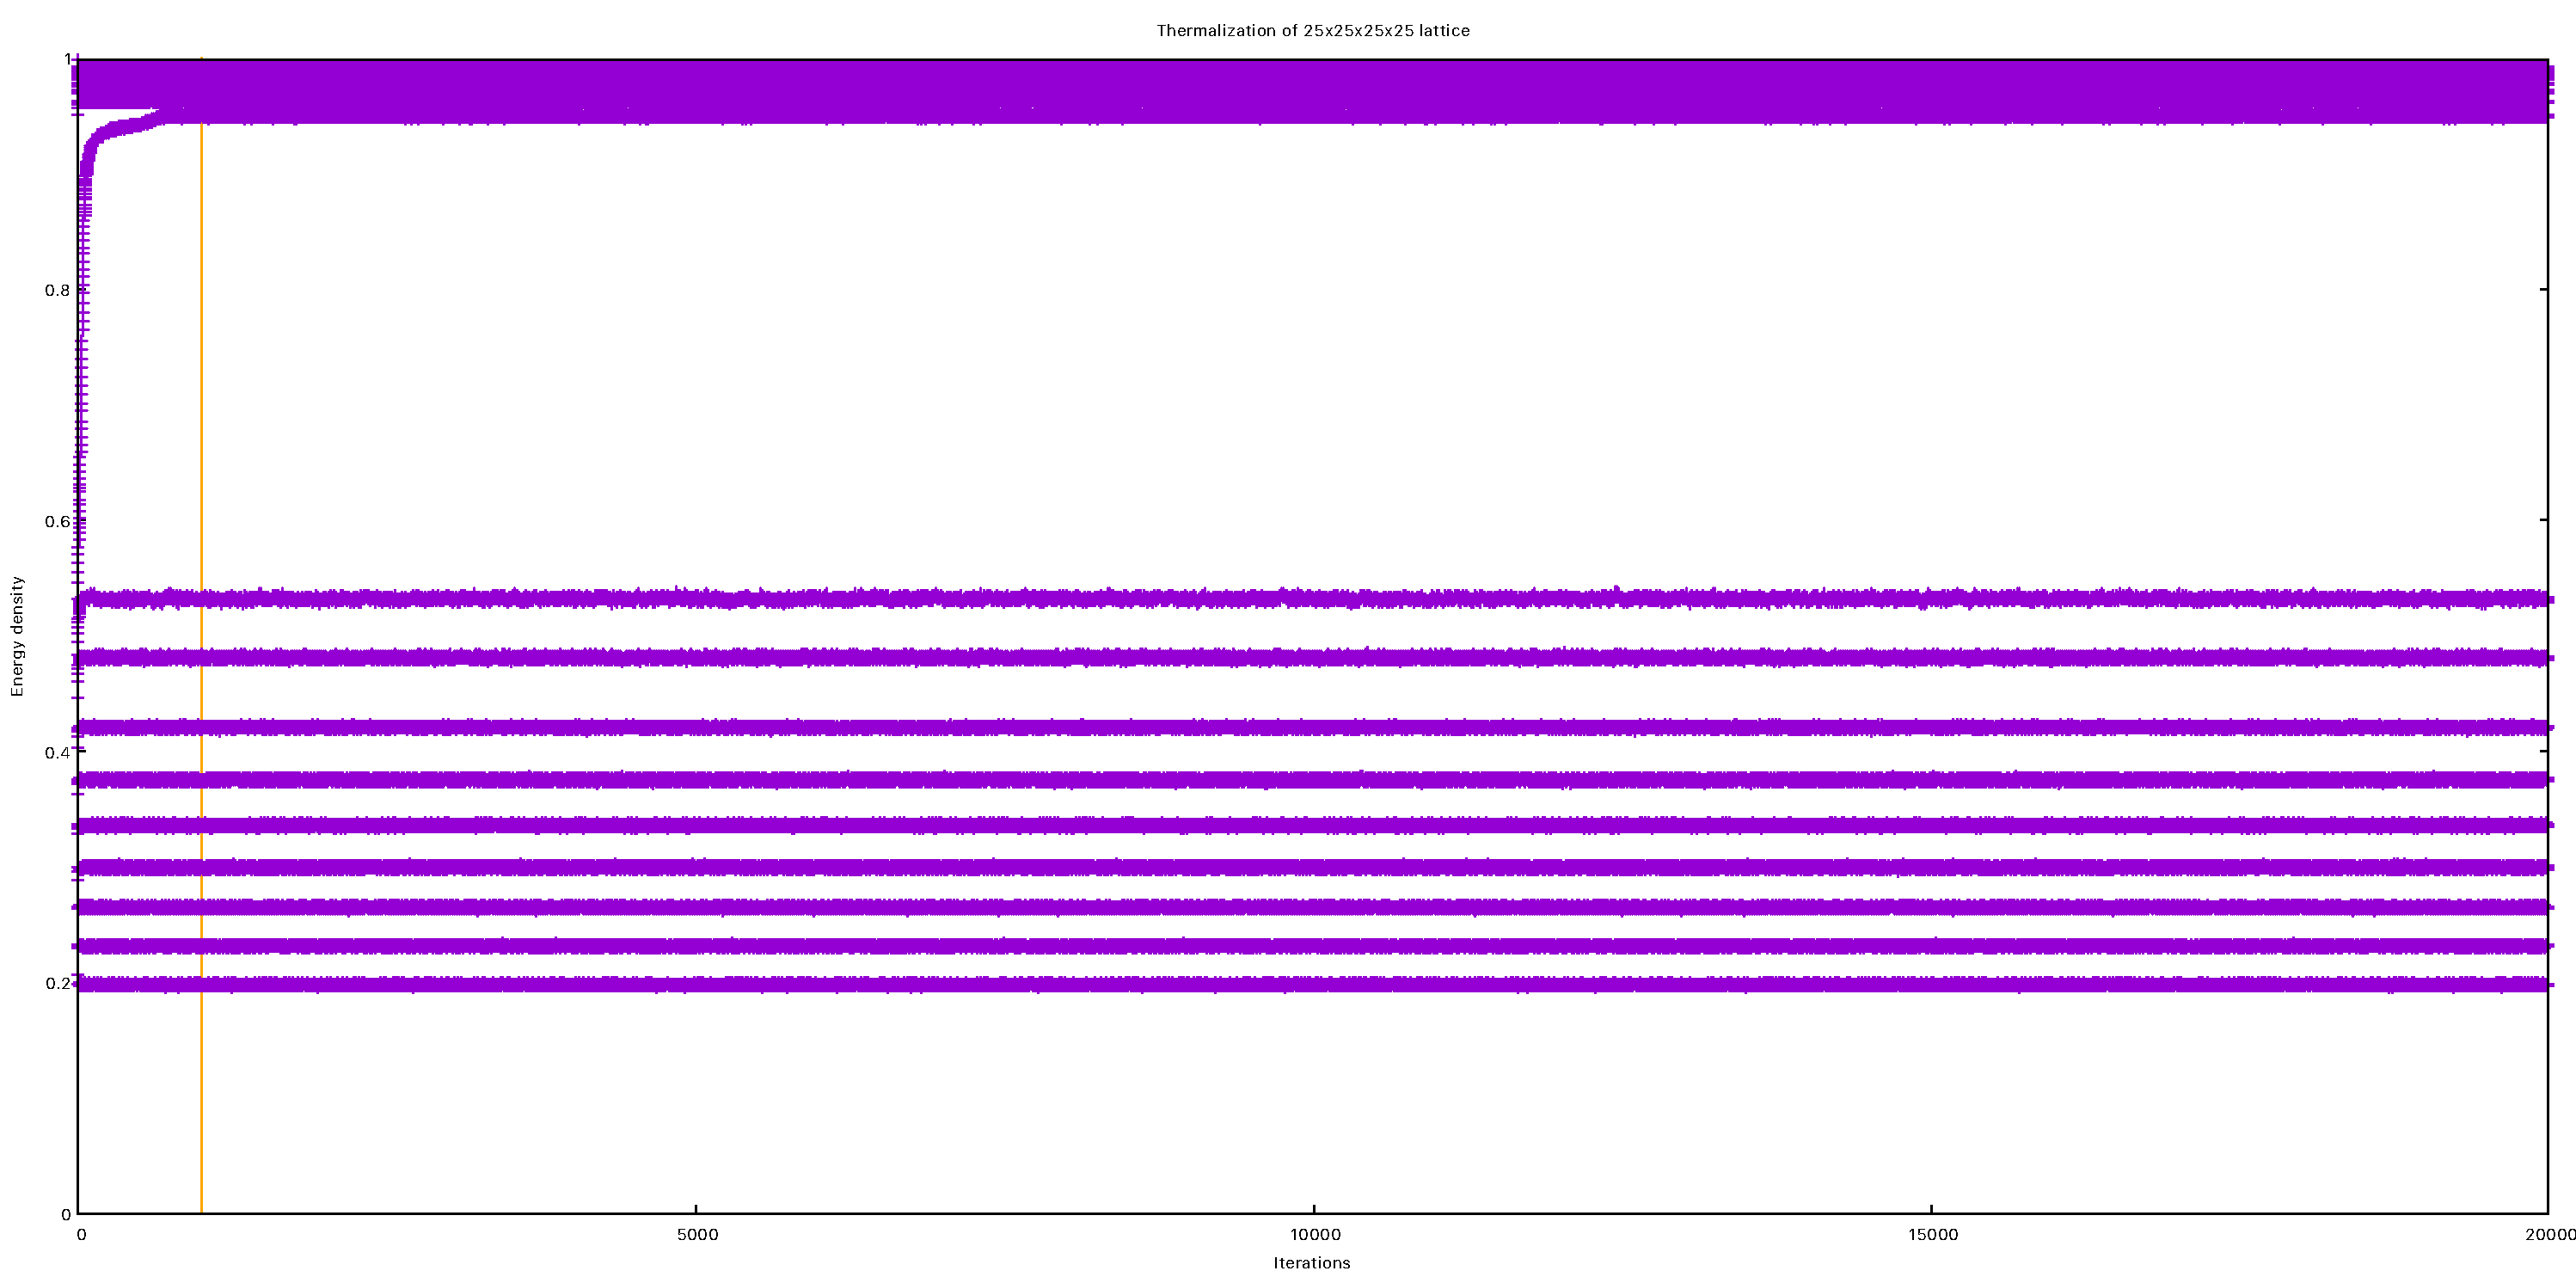
\includegraphics[ scale=0.25 ]{Thermalization252.pdf}
                \caption{Thermalization of 25x25x25x25 lattice gauge system. We will consider "good data" only the right ones with respect the yellow vertical line which
                represent the 1000-th iteration. }
                \label{fig:blocking_energy} 
            \end{figure}
        
        \newpage
        \noindent
        \subsection{Results from blocking}
            \noindent
            As we can observe in \cref{fig:blocking_energy}, \cref{fig:blocking_Wilson} and \ref{fig:blocking_Polyakov} the standard deviation behaves exactly as we predicted.
            \noindent
            \begin{figure}[H]
                \centering
                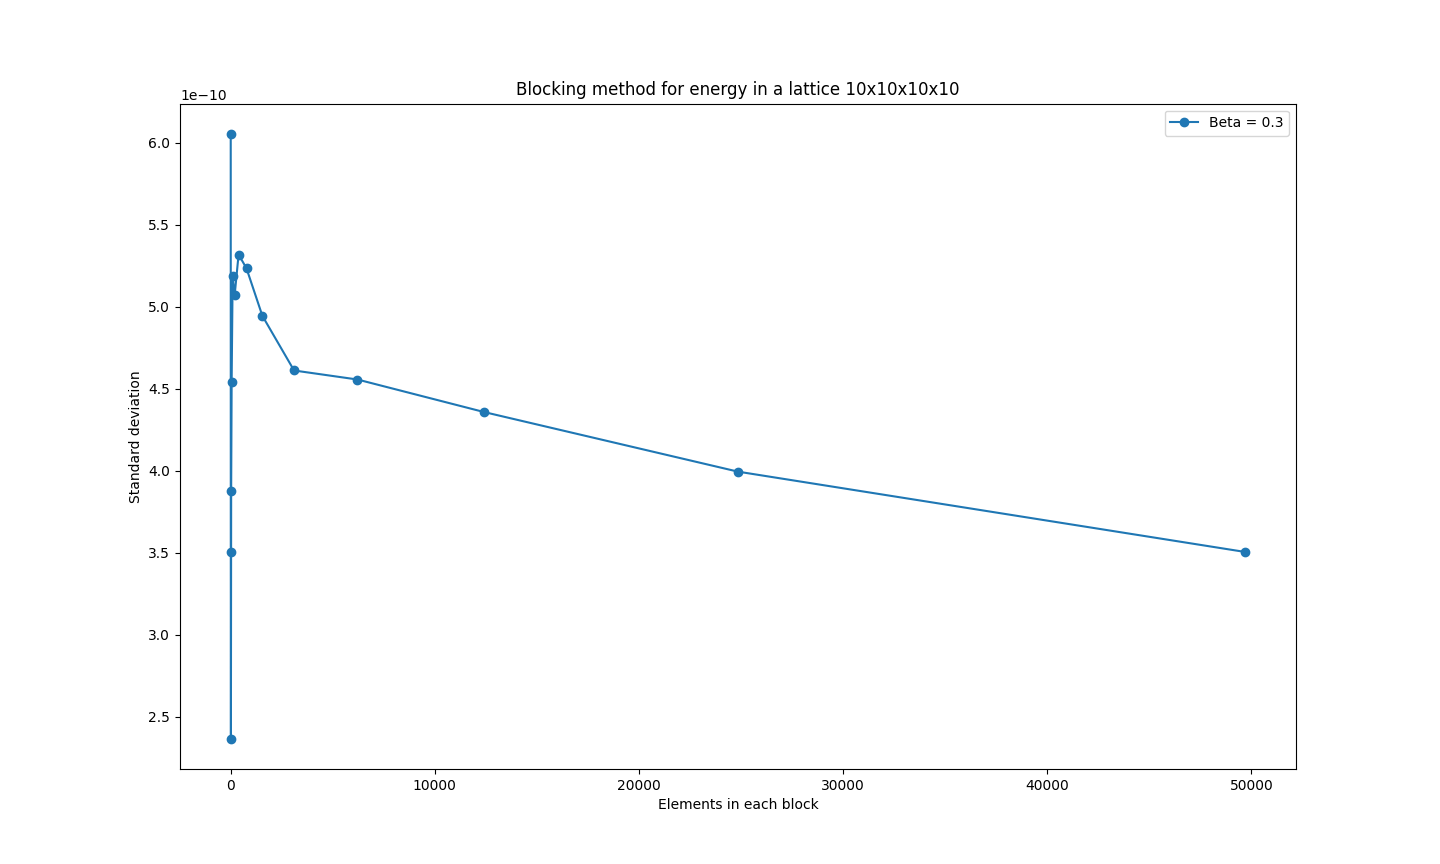
\includegraphics[scale= 0.25]{Blocking_energy.png}
                \caption{Standard deviation for energy density at $\beta=0.3$ by using blocking method.}
                \label{fig:blocking_energy} 
                \includegraphics[scale= 0.25]{blockingWilson.png} 
                \caption{Standard deviation for Wilson loop RxT at $\beta=0.3$ with time distance T=3 and R=3 using blocking method.}
                \label{fig:blocking_Wilson} 
                \includegraphics[scale= 0.25]{BlockingPolyakov.png} 
                \caption{Standard deviation for Polyakov loop at $\beta=0.3$ by using blocking method.}
                \label{fig:blocking_Polyakov} 
                
            \end{figure}
            \noindent
            Too choose the best balance, we used the find\_optimal\_block command in the pyblock library of Python. \\
            However, find\_optimal\_block command choose the best balance in the blocks we get from our dataset, if there are problems in our data, as poor statistics,
            data too much correlated,.. the best block is still not good. \\
            To ensure the goodness of the standard deviation, is important observe if it's properly stabilized by changing the size of the blocks in each dataset.
            \noindent
            \begin{figure}[H]
                \centering
                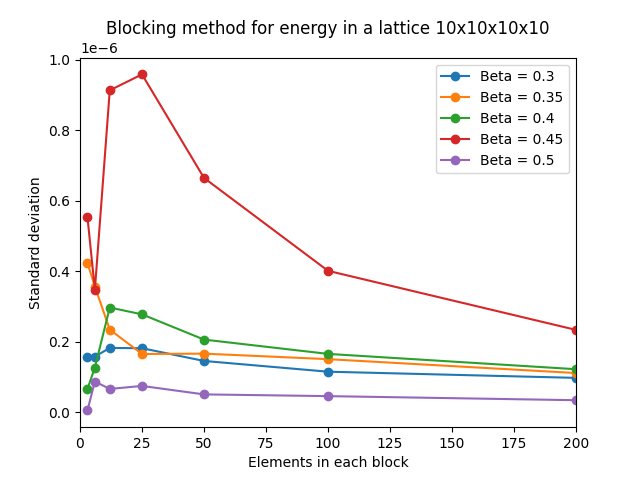
\includegraphics[scale= 0.40]{UncorrectBlocking.png}
                \caption{Standard deviation of density of energy in a 10x10x10x10 lattice. Because of the poor dataset, some standard deviations are not 
                yet properly stabilized.}
                \label{fig:UncorrectBlocking} 
                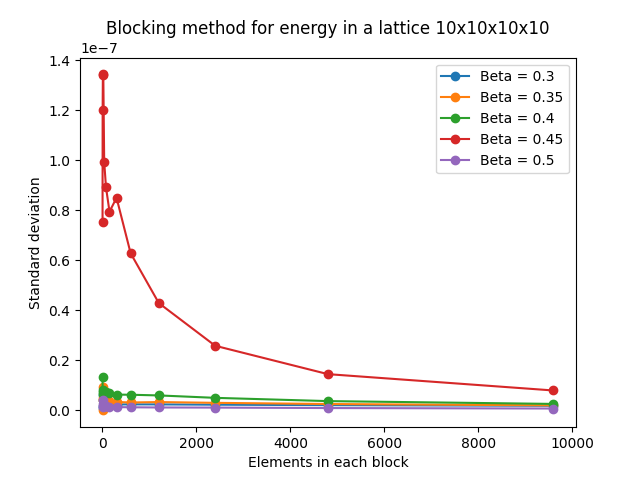
\includegraphics[scale= 0.40]{CorrectBlocking.png} 
                \caption{Standard deviation of density of energy in a 10x10x10x10 lattice. In this case we have more data in each dataset than the 
                \cref{fig:UncorrectBlocking} case.
                In $\beta$=0.45, the standard deviation is higher because it's the dataset in which there is the transition.}
                \label{fig:CorrectBlocking} 
            \end{figure}

            \noindent
            As we can see in \cref{fig:UncorrectBlocking} and in \cref{fig:CorrectBlocking}, the dataset which contain the transition is characterized to an higher
            error.\\
            \noindent 
            The reason of that are the fluctuations, when we approach the transition, the fluctuations increase ( the subset of equilibrium states became bigger ) until 
            allow the transition. Those fluctuations are clearly visible in the observables, which oscillates as a consequence. Now it's clear the reason
            for the higher variance and higher standard deviation as consequence of the dataset near of transitions than the far ones. \\
            \noindent
            For consider this fact without overly burdening the code, we will increase the iterations near the transition and the number of dataset,
            in order to have sufficient statistics also after blocking procedure and confining the transition with more precision.

            \begin{figure}[H]
                \centering
                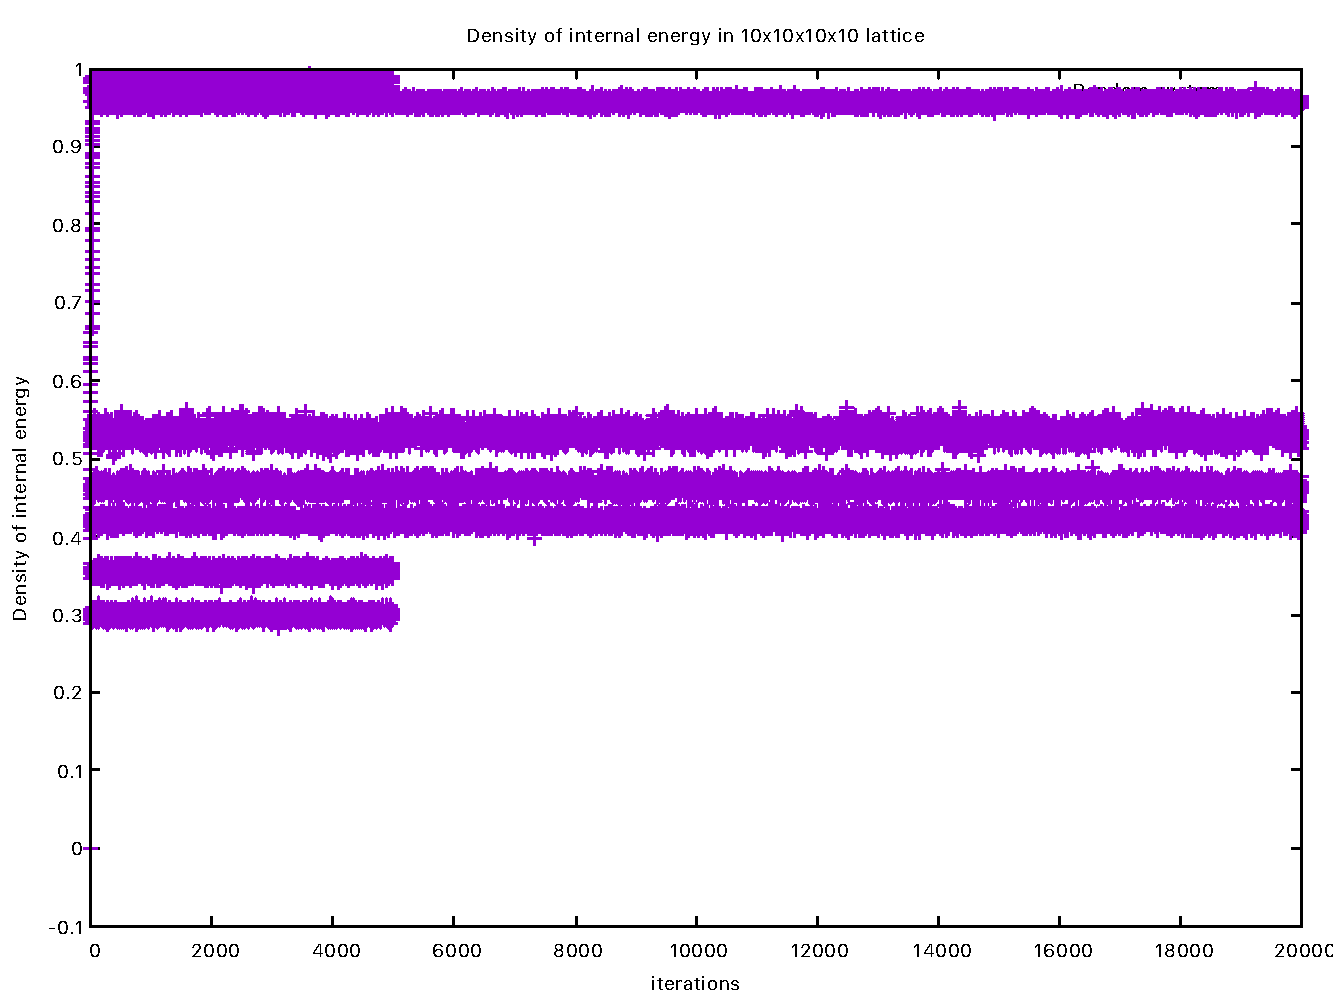
\includegraphics[scale= 0.40]{ThermalizationNotHomogeneous.pdf}
                \caption{In this graph we can observe the 2 lower dataset ( density of internal energy for $\beta$= 0.3 and $\beta$=0.0.35) 
                which contain 5000 iterations, the richer ones in the middle are $\beta$={0.4, 0.425, 0,45, 0.475} and the upper ones $\beta$=0.5 and $\beta$=0.55.}
                \label{fig:NotHomogeneous} 
                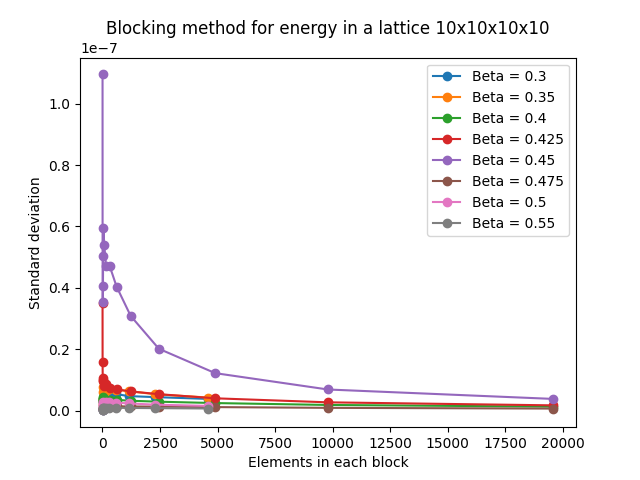
\includegraphics[scale= 0.40]{CorrectBlocking2.png} 
                \caption{Blocking method applied to the dataset represented in \cref{fig:NotHomogeneous}.}
                \label{fig:CorrectBlocking2} 
            \end{figure}
    